\documentclass{sig-alternate}

\usepackage[utf8]{inputenc}
\usepackage{enumitem}
\usepackage[hyphens]{url}
\usepackage[pdftex,urlcolor=black,colorlinks=true,linkcolor=black,citecolor=black,draft]{hyperref}
\def\sectionautorefname{Section}
\def\subsectionautorefname{Subsection}

\usepackage{pifont}

% listings and Verbatim environment
\usepackage{fancyvrb}
\usepackage{relsize}
\usepackage{listings}
\usepackage{verbatim}
\newcommand{\defaultlistingsize}{\fontsize{8pt}{9.5pt}}
\newcommand{\inlinelistingsize}{\fontsize{8pt}{11pt}}
\newcommand{\smalllistingsize}{\fontsize{7.5pt}{9.5pt}}
\newcommand{\listingsize}{\defaultlistingsize}
\RecustomVerbatimCommand{\Verb}{Verb}{fontsize=\inlinelistingsize}
\RecustomVerbatimEnvironment{Verbatim}{Verbatim}{fontsize=\defaultlistingsize}
\lstset{frame=lines,captionpos=b,numberbychapter=false,escapechar=§,
        aboveskip=2em,belowskip=1em,abovecaptionskip=0.5em,belowcaptionskip=0.5em,
        framexbottommargin=-1em,basicstyle=\ttfamily\listingsize\selectfont}

% use Courier from this point onward
\let\oldttdefault\ttdefault
\renewcommand{\ttdefault}{pcr}
\let\oldurl\url
\renewcommand{\url}[1]{\inlinelistingsize\oldurl{#1}}

\lstdefinelanguage{JavaScript}{
  keywords={push, typeof, new, true, false, catch, function, return, null,
    catch, switch, var, if, in, while, do, else, case, break},
  keywordstyle=\bfseries,
  ndkeywords={class, export, boolean, throw, implements, import, this},
  ndkeywordstyle=\color{darkgray}\bfseries,
  identifierstyle=\color{black},
  sensitive=false,
  comment=[l]{//},
  morecomment=[s]{/*}{*/},
  commentstyle=\color{darkgray},
  stringstyle=\color{red},
  morestring=[b]',
  morestring=[b]"
}
\lstset{breaklines=true}

% linewrap symbol
\usepackage{color}
\definecolor{grey}{RGB}{130,130,130}
\newcommand{\linewrap}{\raisebox{-.6ex}{\textcolor{grey}{$\hookleftarrow$}}}

% todo macro
\usepackage{color}
\newcommand{\todo}[1]{\noindent\textcolor{red}{{\bf \{TODO}: #1{\bf \}}}}

% black diamond with white question mark
\usepackage{graphicx,color}
\makeatletter
\newsavebox\Diam@nd \newlength\x@D\newlength\y@D
\newcommand\unknown{%
  \sbox\Diam@nd{\raisebox{-1ex}{\scalebox{1}[1.2]{\rotatebox{45}{\rule{0.8em}{0.8em}}}}}%
  \makebox[\wd\Diam@nd]{\makebox[0pt]{\usebox\Diam@nd}\makebox[0pt]{\textcolor{white}{?}}}}
\makeatother

\hyphenation{WebVTT PageRank}

\newcommand{\vtt}[1]{\texttt{vtt:#1}}
\def\JSONLD{\mbox{JSON-LD}}

\begin{document}
%
% --- Author Metadata here ---
\conferenceinfo{International World Wide Web Conference}{2014 Seoul, Korea}
\CopyrightYear{2014} % Allows default copyright year (20XX) to be over-ridden - IF NEED BE.
%\crdata{0-12345-67-8/90/01}  % Allows default copyright data (0-89791-88-6/97/05) to be over-ridden - IF NEED BE.
% --- End of Author Metadata ---

\title{Weaving the Web(VTT) of Data}

\numberofauthors{6}

\author{
% 1st. author
\alignauthor
Thomas Steiner\titlenote{Second affiliation: \emph{Google Germany GmbH, Hamburg, DE}}\\
       \affaddr{CNRS, Université de Lyon}\\
       \affaddr{LIRIS, UMR5205}\\
       \affaddr{Université Lyon~1, France}\\
       \email{\fontsize{12pt}{14.4pt}\sffamily\selectfont tsteiner@liris.cnrs.fr}
% 2nd. author
\alignauthor
Hannes Mühleisen\\
       \affaddr{Database Architectures Group}\\
       \affaddr{CWI, Science Park 123}\\
       \affaddr{1098 XG Amsterdam, NL}\\
       \email{\fontsize{12pt}{14.4pt}\sffamily\selectfont hannes@cwi.nl}
% 3rd. author
\alignauthor
Ruben Verborgh\\
       \affaddr{Multimedia Lab}\\
       \affaddr{Ghent University -- iMinds}\\
       \affaddr{B-9050 Gent, Belgium}\\
       \email{\fontsize{12pt}{14.4pt}\sffamily\selectfont ruben.verborgh@ugent.be}
\and
% 4th. author
\alignauthor
Pierre-Antoine Champin\\
       \affaddr{CNRS, Université de Lyon}\\
       \affaddr{LIRIS, UMR5205}\\
       \affaddr{Université Lyon~1, France}\\
       \email{\fontsize{12pt}{14.4pt}\sffamily\selectfont pachampin@liris.cnrs.fr}
% 5th. author
\alignauthor
Benoît Encelle\\
       \affaddr{CNRS, Université de Lyon}\\
       \affaddr{LIRIS, UMR5205}\\
       \affaddr{Université Lyon~1, France}\\
       \email{\fontsize{12pt}{14.4pt}\sffamily\selectfont bencelle@liris.cnrs.fr}
% 6th. author
\alignauthor
Yannick Prié\\
       \affaddr{LINA -- UMR 6241 CNRS}\\
       \affaddr{Université de Nantes}\\
       \affaddr{44322 Nantes Cedex 3}\\
       \email{\fontsize{12pt}{14.4pt}\sffamily\selectfont yannick.prie@univ-nantes.fr}
}

\maketitle
\begin{abstract}
Video has become a~first class citizen on the Web
with broad support in all common Web browsers.
Where with structured mark-up on webpages
we have made the vision of the \emph{Web of Data}
a~reality, in this paper, we propose a~new vision
that we name the \emph{Web(VTT) of Data},
alongside with concrete steps to realize this vision.
It is based on the evolving standards \emph{WebVTT}
for adding timed text tracks to videos
and \emph{\JSONLD}, a~JSON-based format to serialize Linked Data.
Just like the \emph{Web of Data}
that is based on the relationships among structured data,
the \emph{Web(VTT) of Data} is based on
relationships among videos based on WebVTT files,
which we use as Web-native spatiotemporal Linked Data containers
with \JSONLD\ payloads.
In a~first step, we provide necessary background information
on the technologies we use.
In a~second step, we perform a~large-scale analysis
of the 148 terabyte size Common Crawl corpus
in order to get a~better understanding
of the \emph{status quo} of Web video deployment
and address the challenge of integrating
the detected videos in the Common Crawl corpus into the
\emph{Web(VTT) of Data}.
In a~third step, we open-source an online video annotation
creation and consumption tool, targeted at videos
not contained in the Common Crawl corpus
and for integrating future video creations,
allowing for weaving the \emph{Web(VTT) of Data}
tighter, video by video.
\end{abstract}

\category{H.5.1}{Multimedia Information Systems}{Video}

%\terms{Experimentation, Design, Standardization}

\vspace{-0.5em}
\keywords{\JSONLD, Linked\thinspace Data, media fragments, Semantic\thinspace Web, video annotation, Web\thinspace of\thinspace Data, WebVTT, Web(VTT)\thinspace of\thinspace Data}

\section{Introduction}

\subsection{From \texttt{\large\textbf{<OBJECT>}} to \texttt{\large\textbf{<video>}}}

In the ``ancient'' times of HTML 4.01~\cite{raggett1999html401},
the \texttt{<OBJECT>} tag\footnote{HTML 4.01 \texttt{<OBJECT>} tag
(uppercased in the spirit of the epoch):
\url{http://www.w3.org/TR/REC-html40/struct/objects.html\#edef-OBJECT}}
was intended for allowing authors to make use of multimedia features
like including images, applets (programs that were automatically downloaded
and ran on the user's machine), video clips, and other HTML documents in their pages.
The tag was seen as a~future-proof all-purpose solution to generic object inclusion.
In an \texttt{<OBJECT>} tag, HTML authors can specify everything required
by an object for its presentation by a user agent:
source code, initial values, and run-time data.
While most user agents have \textit{``built-in mechanisms
for rendering common data types such as text, GIF images,
colors, fonts, and a~handful of graphic elements''},
to render data types they did not support natively---namely videos---%
user agents generally ran external applications and depended on plugins
like Adobe Flash.\footnote{Adobe Flash:
\url{http://get.adobe.com/flashplayer/}}.

While the above paragraph is provocatively written in past tense
and while the \texttt{<object>} tag is still part of both the current
World Wide Web Consortium (W3C) HTML5 specification~\cite{berjon2013html5}
and the Web Hypertext Application Technology Working Group
(WHATWG) ``Living Standard'',%
\footnote{HTML5 \texttt{<object>} tag in the ``Living Standard'' (now lowercased):
\url{http://www.whatwg.org/specs/web-apps/current-work/\#the-object-element}} 
more and more Web video is now powered by the native and well-standardized
\texttt{<video>} tag that no longer depends on plugins.
What currently still hinders the full adoption of \texttt{<video>},
besides some licensing challenges around video codecs,
is its lack of Digital Rights Management (DRM) support
and the fierce debate around it, albeit the Director of the W3C
has confirmed\footnote{New Charter for the HTML Working Group:
\url{http://lists.w3.org/Archives/Public/public-html-admin/2013Sep/0129.html}}
that work in form of the Encrypted Media Extensions~\cite{dorwin2013eme}
on ``playback of protected content '' was in the scope of the HTML Working Group.
However, it can well be said that
HTML5 video has finally become a~first class Web citizen
that all modern browsers fully support.

\subsection{Contributions and Paper Structure}

The paper makes four independent contributions.

\begin{enumerate}[label=\textit{\roman*)},leftmargin=*]
  \item \textbf{The~Vision of the \emph{Web(VTT) of Data}},
  a~global network of videos and connected content
  that is based on relationships among videos based on WebVTT files,
  which we use as Web-native spatiotemporal containers of Linked Data
  with \JSONLD\ payloads.
  \item \textbf{Large-Scale Common Crawl study of the state of Web video:}
    we have examined the 148 terabyte size Common Crawl corpus
    and determined statistics on the usage of the \texttt{<video>},
    \texttt{<track>}, and \texttt{<source>} tags
    and their implications for Linked Data.
  \item \textbf{LinkedVTT conversion tool for WebVTT files:}
  we have made available an on-the-fly online conversion tool
  capable of ``triplifying'' existing WebVTT files
  and any video on YouTube%
  \footnote{YouTube: \url{http://www.youtube.com/}} with closed captions.
  \item \textbf{Online video annotation format and editor:} we have created an
  online video annotation format and an editor prototype implementing it
  that serves for the creation
  and consumption of semantic spatiotemporal video annotations
  turning videos into Linked Data.
\end{enumerate}

The remainder of the paper is structured as follows.
\autoref{sec:technologies-overview} provides an overview
of the enabling technologies that we require for our approach.
\todo{describe paper structure}

\section{Technologies Overview}
\label{sec:technologies-overview}

In this section, we lay the foundations of the set of technologies
that enable our vision of the \emph{Web(VTT) of Data}.
The \texttt{<track>} tag allows authors to specify explicit
external timed text tracks for videos.
With the \texttt{<source>} tag, authors can specify
multiple alternative media resources for a~video.
Both do not represent anything on their own
and are only meaningful as direct child nodes of a~\texttt{<video>} tag.

\paragraph{Web Video Text Tracks format (WebVTT)}

The Web Video Text Tracks format (WebVTT,~\cite{pfeiffer2013webvtt})
is intended for marking up external text track resources mainly
for the purpose of captioning video content.
The recommended file extension is \texttt{vtt},
the MIME type is \texttt{text/vtt}.
WebVTT files are encoded in UTF-8 and
start with the required string \texttt{WEBVTT}.
Each file consists of items called \emph{cues}
that are separated by an empty line.
Each cue has a~start time and an end time in
\texttt{hh:mm:ss.milliseconds} format,
separated by a~stylized ASCII arrow \texttt{-}\texttt{->}.
The cue payload follows in the line after the cue timings part
and can span multiple lines.
Typically, the cue payload contains plain text,
but can also contain textual data serialization formats like JSON,
which later on in the paper we will show is essential
for our proposed approach to semantic video annotation.
%Spans of text associated with a~specific voice can be annotated
%in form of WebVTT cue voice spans.
%A~WebVTT voice tag, denoted by \texttt{<v VOICE>}, has a~value,
%which is the name of the voice.
Cues optionally can have unique WebVTT identifiers.
WebVTT-compliant Web browsers~\cite{dutton2012trackelement}
support five different kinds of
WebVTT tracks: \texttt{subtitles}, \texttt{captions},
\texttt{descriptions}, \texttt{chapters}, and \texttt{metadata},
detailed in \autoref{table:texttrackkinds}
and specified in HTML5~\cite{berjon2013html5}.
In this paper, we focus on
text tracks of kind \texttt{metadata}
meant to be used from a~scripting context and
not displayed by user agents.

\begin{table}[b!]\footnotesize
\begin{tabular}{ r p{5.5cm} } % ACM column width 8.45cm, 0.83cm gutter
\textbf{WebVTT Kind} & \textbf{Description and Default Behavior}\\

\texttt{subtitles} & Transcription or translation of speech,
suitable for when sound is available but not understood.
Overlaid on the video.\\

\texttt{captions} & Transcription or translation of the dialogue,
sound effects, and other relevant audio information,
suitable for when sound is unavailable or not clearly audible.
Overlaid on the video;
labeled as appropriate for the hard-of-hearing.\\

\texttt{descriptions} & Textual descriptions of the video component
of the media resource, intended for audio synthesis
when the visual component is obscured, unavailable, or unusable.
Synthesized as audio.\\

\texttt{chapters} & Chapter titles, intended to be used for navigating
the media resource. Displayed as an interactive (potentially nested)
list in the user agent's interface.\\

\texttt{metadata} & Metadata intended for use from script context.
Not displayed by user agent.\\
\end{tabular}
  \caption{WebVTT text track kinds in HTML5~\cite{berjon2013html5}}
  \label{table:texttrackkinds}
\end{table}

For scripting purposes, the video element
has a~property called \texttt{textTracks}
that returns a~\texttt{TextTrackList} of
\texttt{TextTrack} members, each of which correspond
to track elements.
A~\texttt{TextTrack} has a~\texttt{cues} property
that returns a~\texttt{TextTrackCueList} of individual
\texttt{TextTrackCue} items.
Cue data is accessible via properties like
\texttt{startTime} and \texttt{endTime} and,
most importantly, \texttt{text} to obtain a~cue's payload.
When the payload is in JSON format,
it can be parsed via the
\texttt{JSON.parse()} function in JavaScript.
When a~video is playing,
JavaScript events of the \texttt{TextTrack} and \texttt{TextTrackCue}
elements fire automatically when the \texttt{currentTime}
of the video matches
a~cue's \texttt{startTime} or \texttt{endTime}.
\texttt{TextTrack} elements fire \texttt{oncuechange} events,
whereas \texttt{TextTrackCue} elements fire
\texttt{onenter} and \texttt{onexit} events.
JavaScript applications can subscribe to these events.
Important for us, both \texttt{TextTrack} and
\texttt{TextTrackCue} elements
can be dynamically generated via JavaScript.

\paragraph{\JSONLD}

The \emph{JavaScript Object Notation}%
\footnote{JavaScript Object Notation: \url{http://json.org/}}
(JSON)
is a~(despite the name) language-independent textual syntax
for serializing objects, arrays, numbers, strings, booleans, and null.
\emph{Linked Data}~\cite{bizer2009linkeddata}
describes a~method of publishing structured data
so that it can be interlinked and become more useful,
which builds upon standard Web technologies such as HTTP, RDF and URIs.
Based on top of JSON, the
\emph{JavaScript Object Notation for Linked Data}
(\JSONLD,~\cite{sporny2013jsonld}) is a~method for transporting
Linked Data with a~smooth upgrade path from JSON to \JSONLD.
\JSONLD\ properties like \texttt{title} can be mapped to taxonomic
concepts (like \texttt{dc:title} from Dublin Core%
\footnote{Dublin Core: \url{http://dublincore.org/documents/dces/}})
via so-called data contexts.

\paragraph{Media Fragments URI}

Media Fragments URI~\cite{troncy2012mediafragments}
specifies a~syntax for constructing URIs of media fragments
and explains how to handle them over the HTTP protocol.
The syntax is based on the specification of
name-value pairs that can be used in URI query strings
and URI fragment identifiers to restrict a~media resource
to a~certain fragment.
Media Fragments URI supports temporal and spatial media fragments.
The \emph{temporal dimension} is denoted
by the parameter name \texttt{t} and specified
as a~half-open interval with begin time and end time
that may also be omitted,
with the begin time defaulting to 0 seconds
and the end time defaulting to the media item's duration.
The \emph{spatial dimension} selects
a~rectangular area of pixels from media items.
Rectangles can be specified as pixel coordinates or percentages.
Rectangle selection is denoted by the parameter name \texttt{xywh}.
The value is either \texttt{pixel:} or \texttt{percent:}
(defaulting to \texttt{pixel:})
followed by four comma-separated integers.
The integers denote $x$, $y$, $width$, and $height$ respectively,
with $x = 0$ and $y = 0$ being the top left corner of the media item.
If \texttt{percent:} is used, $x$ and $width$ are interpreted
as a~percentage of the width of the original media item,
$y$ and $height$
of the original height.

\paragraph{Ontology for Media Resources}

The Ontology for Media Resources~\cite{lee2012mediaontology}
serves to bridge different description methods of media resources
and to provide a~core set of descriptive properties.
It also defines mappings to common metadata formats.
Combined with Media Fragments URI,
this allows for making ontologically anchored statements
about media items and fragments thereof.

\section{Large-Scale Common Crawl\\ Study of the State of Web Video}

Part of the objectives behind the \emph{Web(VTT) of Data}
is to create a~truly interconnected global network of and between videos
containing Linked Data pointers to related content of all sorts,
where diverse views are not filtered by the network bubble, 
but where serendipitously new views can be discovered
by taking untrodden Linked Data paths.
In order to get there,
we have conducted a~large-scale study
based on the Common Crawl corpus to get a~better understanding
of the \emph{status quo} of Web video and timed text track deployment.

\subsection{Common Crawl}

The Common Crawl Foundation\footnote{Common Crawl: \url{http://commoncrawl.org/}}
is a~non-profit organization founded in 2008 by Gil Elbaz.
Its objective is to democratize access to Web information
by producing and maintaining an open repository of Web crawl data
that is universally accessible and analyzable~\cite{simonite2013commoncrawl}.
All Common Crawl data is stored on Amazon Simple Storage Service (Amazon~S3)%
\footnote{Amazon S3: \url{http://aws.amazon.com/s3/}} and
accessible to anyone via Amazon Elastic Compute Cloud (Amazon~EC2),%
\footnote{Amazon EC2: \url{http://aws.amazon.com/ec2/}}
allowing the data to be downloaded in bulk,
as well as directly be accessed for map-reduce processing in EC2.
The, at time of writing, latest dataset was collected at the end of 2013,
contains approximately 2.3~billion webpages
and is 148 terabyte in size~\cite{green2014winter}.
Crawl raw data is stored in the Web ARChive format
(WARC,~\cite{iso285002008warc}), an evolution of the previously used
Archive File Format (ARC,~\cite{burner1996arc}),
which was developed at the Internet Archive.%
\footnote{Internet Archive: \url{https://archive.org/}}
Each crawl run is hierarchically organized in segments directories
that contain the WARC files with the HTTP requests and responses for each fetch,
and individual Web Archive Metadata (WAT,~\cite{goel2011wat}) files,
which describe the metadata of each request and response.
While the Common Crawl corpus gets bigger with each crawl run,
it obviously does not represent the ``whole Web'',
which is an illusive concept anyway,
given that a~simple calendar Web application can produce an infinite number of pages.
Common Crawl decides on the to-be-included pages based on an implementation%
\footnote{Common Crawl PageRank code:
\url{https://github.com/commoncrawl/commoncrawl-crawler/tree/master/src/org/commoncrawl/service/pagerank}}
of the PageRank~\cite{page1999pagerank} algorithm,
albeit the inclusion strategy is unknown---%
despite the foundation's focus on transparency.

\subsection{On the Quest for WebVTT}

We have analyzed the entire 148 terabytes of crawl data
using an Elastic Compute Cloud job
whose code was made available as open-source.%
\footnote{EC2 job:
\url{https://github.com/tomayac/postdoc/blob/master/demos/warczenschwein/src/main/java/com/tomayac/warczenschwein/TagTool.java}}
Rather than parse each document as HTML,
we have tested them for the regular expression
\texttt{<video[\^{}>]*>(.*?)</video>},
an approach that also in previous experiments
proved very efficient%
~\cite{bizer2013deployment,muhleisen2012web}.
We tested exactly 2,247,615,323 webpages
that had returned a successful HTTP response to the Common Crawl bot,
and had to skip exactly 46,524,336  non-HTML documents.
On these webpages, we detected exactly
2,963,766 \texttt{<video>} tags,
resulting in a~1.37 gigabyte raw text file
that we have made available publicly.%
\footnote{2,963,766 \texttt{<video>} tags: \url{https://drive.google.com/file/d/0B9LlSNwL2H8YdWVIQmJDaE81UEk}}
This means that on average only ${\approx}0.132\%$ of all webpages contain video.
The whole job took about five hours on
80~c1.xlarge machines and costed overall \$555,
consisting of \$468 for Amazon~EC2,
plus an additional \$87 for Amazon Elastic MapReduce
 (Amazon EMR)\footnote{Amazon EMR:
\url{http://aws.amazon.com/elasticmapreduce/}}

\subsection{Text Track Statistics}
\label{sec:text-track-statistics}

From all 2,963,766 \texttt{<video>} tags,
only 1,456 (${\approx0.049\%}$) had a~\texttt{<track>} child node.
Upon closer examination of the kinds of these 1,456 \texttt{<track>} nodes
(see \autoref{table:texttrackkinds} for an explanation of the various kinds),
we saw that the overwhelming majority are unsurprisingly
used for \texttt{subtitles} or \texttt{captions}.
Almost no \texttt{chapter} usage was detected
and neither \texttt{metadata} nor \texttt{description} usage at all.
The full details can be seen in \autoref{table:kind}.
Looking at the languages used in the captions and subtitles, 
these were almost exclusively English and French,
as can be seen in \autoref{table:srclang}.
The track labels listed in \autoref{table:label}
indeed confirm this observation.
In case of multiple tracks for one video,
one track can be marked as the default track.
This happens through a~boolean attribute,%
\footnote{HTML boolean attributes:
\url{http://www.whatwg.org/specs/web-apps/current-work/\#boolean-attributes}}
whose value either needs to be the empty string
or the attribute's name,
which is ``default'' in the concrete case.
\autoref{table:default}
shows that this was used correctly in almost all cases.
When we tried to determine the MIME type of the actual
text tracks, we relied on the file extension
of the values given in the \texttt{<track src>} attributes.
As a~significant amount of text tracks
seems to be dynamically generated on-the-fly---%
and thus had no file extension but a~video identifier in the URL instead---%
we used an approximation to check if some part
of the URL matched the regular expression \texttt{/\textbackslash bvtt\textbackslash b/gi}.
Based on this approximation,
a~little over half of all text tracks
are in WebVTT format
with the extension \texttt{.vtt}
or rarely \texttt{.webvtt}.
The predecessor SubRip file format%
\footnote{SubRip file format:
\url{http://www.matroska.org/technical/specs/subtitles/srt.html}}
can still be encountered in about
a~quarter of all text tracks.
The full details are available in \autoref{table:src}.
Almost all videos had only exactly one text track
rather than multiple, as detailed in \autoref{table:track},
meaning that the broad majority of all videos are subtitled or captioned
in only one language, English or French (\autoref{table:srclang}).

\subsection{Video Statistics}

As in \autoref{sec:online-video-annotation-format-and-editor}
we will report on ways to make semantic statements
about videos on the Web,
we have additionally compiled some video statistics.
Unlike with images on the Web, where
semantic statements in
Resource Description Framework (RDF)
can be made based on the image's
URL~\cite{linsley2009rdfa},
with Web video, the situation is another.
Due to different Web browsers supporting
different video codecs,
it is a~common practice to provide videos
in different encodings.
The user's Web browser then dynamically selects
a~version it can play.
This is realized through the \texttt{<source>} tag.
\autoref{table:source} shows the observed numbers of
\texttt{<source>} tag child nodes per
\texttt{<video>} tag \emph{with} \texttt{<track>} tag,
with the result that up to
four sources are given for essentially the ``same'' video.
\autoref{table:sourceFull} confirms this observation
for the entire collection of all \texttt{<video>} tags
\emph{with or without} \texttt{<track>} tag.
\autoref{table:type} shows the distribution
of values for the \texttt{<source type>} attribute
of \texttt{<video>} tags \emph{with} \texttt{<track>} tag,
the clear leaders being the MP4 format
followed by WebM,
a~trend that again is also reflected
in \autoref{table:typeFull}
within the entire collection
of all \texttt{<video>} tags
\emph{with or without} \texttt{<track>} tag.

\subsection{Implications on Linked Data for Videos}
\label{sec:implications-on-linked-data-for-videos}

The biggest issue with this practice
of putting multiple sources is that
rather than having one unique identifier (URL) per video,
there can be multiple identifiers.
\autoref{listing:html-license} shows a~minimal example.
Unless one repeats all statements for each source,
there will always remain unclear sources without structured data.
We note that a~video in encoding~A
and the ``same'' video in encoding~B
may not be marked as \texttt{<owl:sameAs>},
because statements about the encoding format
of one video do not apply to the other,
the identity symmetry condition would thus be violated.
In practice, a~solution similar to
specifying canonical URLs in Web search%
~\cite{kupke2009canonical} seems feasible.
Another approach is to require a~unique identifier
in the \texttt{<video id>} attribute,
which allows for addressing the video
with fragment identifiers.
More advanced approaches to the problem
stemming from the bibliographic universe
like FRBR~\cite{tillett2004frbr} are possible,
but for the concrete use case seem quite complex.

\begin{lstlisting}[caption={Specifying a~license for an image and attempt to do the same for a~video with two sources (the license of kitten.webm stays unclear)},
  label=listing:html-license, language=html, float=t!]
<div about="kitten.jpg">
  <img src="kitten.jpg" alt="Cute kitten" />
  <a rel="license" href="http://creativecommons.org/licenses/by-sa/3.0/">
    Creative Commons Attribution Share-Alike 3.0
  </a>
</div>

<div about="kitten.mp4">
  <video>
    <source src="kitten.mp4"/>
    <source src="kitten.webm"/>
  </video>  
  <a rel="license" href="http://creativecommons.org/licenses/by-sa/3.0/">
    Creative Commons Attribution Share-Alike 3.0
  </a>
</div>
\end{lstlisting}

\section{LinkedVTT Conversion Tool for WebVTT Files}
\label{sec:linkedvtt-conversion-tool-for-webvtt-files}

The WebVTT specification~\cite{pfeiffer2013webvtt} defines a~syntax
for conveying timed video text tracks,
and a~semantics for this syntax in terms of how
Web browsers should process such tracks.
It achieves this by specifying an underlying data model for those tracks.
The aim of this section is to show
how this data model can easily be mapped to RDF-based Linked Data,
and thus allowing for many other usage scenarios for this data.
For this purpose, we propose an RDF-Schema ontology%
\footnote{RDF-Schema ontology:
\url{http://champin.net/2014/linkedvtt/onto\#}}
conveying the WebVTT data model.
In the rest of the paper, terms from this ontology
will be preceded by the \vtt{} prefix.
An online implementation of this interpretation process
that we have titled LinkedVTT is likewise available online.%
\footnote{LinkedVTT: \url{http://champin.net/2014/linkedvtt/}}
It takes the URL of any WebVTT file, the contents of a~raw WebVTT file,
or a~YouTube URL of any video with closed captions as an input,
and applies the conversion from WebVTT to Linked Data on-the-fly.

\subsection{Basic Interpretation}

A WebVTT file defines a~set of cues,
which are described by a~pair of timestamps and a~payload.
In other words, each cue is an annotation of the video,
associating a~temporal video fragment to the payload,
delimited by the two timestamps.
As there is a~standard way of identifying \emph{temporal}
and \emph{spatial} video fragments
with a~URI~\cite{troncy2012mediafragments}
it is straightforward to represent this annotation as an RDF triple.
We therefore propose a~property \vtt{annotatedBy}
to serve as predicate for those triples.
To keep the context of each annotation,
we use the notion of RDF dataset~\cite{cyganiak2014rdf11concepts}.
Each \vtt{annotatedBy} triple is enclosed in a~named graph,
whose name is either a~URI, based on the cue identifier if it has one,
or a~blank node if the cue has no identifier.
The default graph of the dataset describes its overall structure,
linking the dataset URI to all the URIs and blank nodes identifying its cues
with the \vtt{hasCue} property.
In the default graph, each cue is also linked to
the Media Fragment URI it describes,
with the \vtt{describesFragment} property. 
As the notion of dataset is a recent addition to the RDF core concepts
(previously, it was specific to the SPARQL query language),
we envision that some consumers will not be able to deal with it.
Hence we propose an alternate interpretation of WebVTT as RDF.
In this so-called \emph{flat} interpretation,
the contents of all named graphs is merged into the default graph.

\subsection{Advanced Interpretation}

WebVTT is not limited to textual timed text tracks.
As \autoref{table:texttrackkinds} details, the HTML5
\texttt{<track>} tag supports different kinds of tracks,
one of them being \textit{metadata},
a~track designed for machine rather than human consumption.
Although it was shown in \autoref{sec:text-track-statistics}
that there is no measurable evidence of use for this kind of track yet---%
which is understandable given that the technology
is still under development---%
we propose that JSON data is a~good candidate for cues of such tracks.
JSON has a~textual syntax that is easy to author
and easy to process in a~Web browser and elsewhere.
Furthermore, \JSONLD~\cite{sporny2013jsonld} provides
a~standard way to interpret JSON data as Linked Data,
which fits nicely with our approach.
More precisely, whenever the payload of a~cue
successfully parses as a~JSON object,
we consider that this object is meant to
represent the annotated media fragment itself,
and interpret it as \JSONLD.
In consequence, all properties of the JSON object
are applied directly to the fragment,
and embedded structures can be used to describe
other resources related to that fragment,
\emph{e.g.}, depicted persons, locations, topics, related videos
or video fragments, or spatiotemporal video tags.
In this case, all the triples generated from parsing the payload as \JSONLD\
\emph{replace} the \vtt{annotatedBy} triple in the cue's named graph.
\autoref{listing:webvtt} gives an example of such \JSONLD\ payload.
We note that \JSONLD\ requires a~\emph{context}
to interpret JSON data as Linked Data,
especially to disambiguate keywords to full URIs.
This context can be provided in each cue,
but in the following we also provide an alternative way to declare it once
for the entire WebVTT file.

\begin{comment}
\begin{lstlisting}[caption={A~WebVTT cue with a~\JSONLD\ payload},
  label=listing:jsonld-payload, float=t!]
00:00:00.000 --> 00:00:12.000
{
  "label": "Vince and Jules in the car",
  "depicts": [
    {
      "@id": "http://wikidata.org/entity/Q80938",
      "name": "John Travolta"
    },
    {
      "@id": "http://wikidata.org/entity/Q172678",
      "name": "Samuel L. Jackson"
    }
  ]
}
\end{lstlisting}
\end{comment}

\begin{lstlisting}[caption={Sample WebVTT metadata file with \JSONLD\
  payload in a~cue identified as ``cue1''},
  label=listing:webvtt, float=t!]
WEBVTT

cue1
00:00:00.000 --> 00:00:12.000
{
  "@context": "http://ex.org/local_context",
  "tags": ["wind scene", "opening credits"],
  "contributors": ["http://ex.org/sintel"]
}
\end{lstlisting}

\subsection{Linked Data Related Metadata}

In addition to the cues, WebVTT files can contain
metadata headers described as key-value pairs.
While the WebVTT specification defines a~number of metadata headers,
it leaves it open for extensions.
We propose three extended metadata headers listed below.
Most WebVTT currently does not contain
these metadata headers,
but we argue that they allow for an easy transition
from plain WebVTT to Linked Data WebVTT,
just like \JSONLD\ makes it easy to turn plain JSON into Linked Data
by adding a \texttt{@context} property.

\begin{description}
  \item[@base]
  Sets the base URI used for resolving relative URIs.
  This applies to any relative URIs that would be found in the \JSONLD\ descriptions,
  but also to generate URIs for cues based on their identifiers.
  It defaults to the URI of the WebVTT file.
  \item[@context]
  This key can be used multiple times; each value is the URI
  of a~\JSONLD\ context that should be used to
  interpret the JSON payloads in the WebVTT file.
  \item[@video]
  Sets the URI for the video for generating media fragment URIs.
  If not present, the video URI must be provided externally,
  \emph{e.g.}, the \texttt{<video src>} attribute of the video
  containing the WebVTT track.
  This metadata header is a~direct response to an issue that we
  have outlined in \autoref{sec:implications-on-linked-data-for-videos}.
\end{description}

\subsection{Integrating Existing Videos Into the\\ Web(VTT) of Data}

Given the currently rather manageable amount of videos
with captions or subtitles as outlined in \autoref{sec:text-track-statistics},
approaches for the automated semantic lifting
based on timed text track data are feasible. 
These approaches extract the transcribed text snippets from cues
and either convert them into one consistent block of text
or treat each text snippet in isolation
before applying named entity extraction on them.
Typical examples are~\cite{li2013enriching,li2012creating,yi2012synote}
by Li \emph{et~al.}\ and~\cite{steiner2010semwebvid} by us.
In combination with Media Fragments URI, spatiotemporal annotations
can be created on-the-fly with good precision.

\begin{table}[p!]
  \raggedleft
  \begin{tabular}{ r | r }                       
    \texttt{<track kind>} & Count \\
    \hline  
    captions & 915\\
    subtitles & 525\\
    chapters & 2\\
    description & 0\\
    metadata & 0\\
    undefined & 10\\  
  \end{tabular}
  \caption{Distribution of values for
    \texttt{<track kind>}}
  \label{table:kind}
\end{table}

\begin{table}[p!]
  \raggedleft
  \begin{tabular}{ r | r }                       
    \texttt{<track srclang>} & Count \\
    \hline  
    en & 1,242\\
    fr & 117\\
    de & 8\\    
    en-US & 3\\
    th & 2\\
    Español & 1\\
    Korean & 1\\
    undefined & 78\\    
  \end{tabular}
  \caption{Distribution of values for
    \texttt{<track srclang>}}
  \label{table:srclang}    
\end{table}

\begin{table}[p!]
  \raggedleft
  \begin{tabular}{ r | r }                       
    \texttt{<track label>} & Count \\
    \hline  
    English & 1,069\\
    Français & 117\\    
    English Captions & 20\\    
    Captions & 10\\
    English closed captioning & 3\\    
    Deutsch & 2\\    
    English Subtitles & 2\\
    Thai & 2\\    
    English subtitles & 1\\
    Gr\unknown\unknown e & 1\\
    undefined & 229\\
  \end{tabular}
  \caption{Distribution of values for
    \texttt{<track label>} \tiny (unknown encoding \emph{sic})}
  \label{table:label}    
\end{table}
  
\begin{table}[p!]
  \raggedleft
  \begin{tabular}{ r | r }                       
    \texttt{<track default>} & Count \\
    \hline
    default & 650\\
    `' & 526\\
    true & 1\\
    undefined & 279
  \end{tabular}
  \caption{Distribution of values for
    \texttt{<track default>}}
  \label{table:default}    
\end{table}

\begin{table}[p!]
  \raggedleft
  \begin{tabular}{ r | r }                       
    File extensions of \texttt{<track src>} & Count \\
    \hline
    probably \texttt{.vtt} & 696\\
    \texttt{.srt} & 390\\
    \texttt{.vtt} or \texttt{.webvtt} & 66\\
    no extension & 304\\
  \end{tabular}
  \caption{Distribution of file extensions for
    values for \texttt{<track src>}}
  \label{table:src}    
\end{table}

\begin{table}[p!]
  \raggedleft
  \begin{tabular}{ r | r }                       
    \texttt{<track>} tags & Count \\
    \hline
    1 & 1,446\\
    0 & 9\\
    9 & 1\\
  \end{tabular}
  \caption{Number of \texttt{<track>} tags per
    \texttt{<video>} tag \tiny (zero \texttt{<track>}
    tags means  the \texttt{<video>} tag had
    an  unparseable \texttt{<track>})}
  \label{table:track}    
\end{table}

\begin{table}[p!]
  \raggedleft
  \begin{tabular}{ r | r }
    \texttt{<source>} tags & Count \\
    \hline
    1 & 826\\    
    3 & 404\\    
    2 & 173\\    
    0 & 49\\
    4 & 4\\
  \end{tabular}
  \caption{Number of \texttt{<source>} tags per
    \texttt{<video>} with \texttt{<track>} \tiny (zero \texttt{<source>}
    tags means the video URL was provided via
    \texttt{<video src>}; 1,405 videos did not have
    a~\texttt{src} attribute, 51 videos had one)}
  \label{table:source}    
\end{table}

\begin{table}[p!]
  \raggedleft
  \begin{tabular}{ r | r }
    \texttt{<source>} tags & Count \\
    \hline
    0 & 7,828,032\\
    1 & 1,139,240\\
    3 & 138,540\\
    4 & 83,121\\    
    2 & 77,853\\
    6 & 804\\    
    5 & 179\\
    7 & 137\\
    8 & 64\\
    10 & 22\\    
    9 & 9\\
    13 & 8\\
    11 & 6\\
  \end{tabular}
  \caption{Number of \texttt{<source>} tags per
    \texttt{<video>} with or without \texttt{<track>}
    \tiny (zero \texttt{<source>}
    tags means the video URL was provided via
    \texttt{<video src>})}
  \label{table:sourceFull}    
\end{table}

\begin{table}[p!]
  \raggedleft
  \begin{tabular}{ r | r }
    \texttt{<source type>} & Count \\
    \hline
    video/mp4 & 1,285\\
    video/webm & 94\\
    video/x-ms-wmv & 10\\    
    video/ogg & 5\\    
    video/mp4; codecs=``avc1.42E01E, mp4a.40.2'' & 3\\
    video/flv & 2\\
    video/youtube & 1\\    
    undefined & 58\\  
  \end{tabular}
  \caption{Distribution of values for \texttt{<source type>}
    of \texttt{<video>} tags with \texttt{<track>}}
  \label{table:type}    
\end{table}

\begin{table}[p!]
  \raggedleft
  \begin{tabular}{ r | r }
    \texttt{<source type>} & Count \\
    \hline
    video/mp4 & 1,204,744\\
    video/webm & 163,715\\
    video/mp4; codecs="avc1.42E01E, mp4a.40.2" & 10,700\\
    text/json & 2,841\\
    video/flv & 2,281\\
    video/x-ms-wmv & 2,105\\
    video/flash & 2,023\\
    video/ogg & 1,529\\
    video/youtube & 1,528\\
    application/x-mpegURL & 1,257\\    
  \end{tabular}
  \caption{Distribution of values for \texttt{<source type>}
    of \texttt{<video>} tags with or without  \texttt{<track>}
    \tiny (with more than 1,000 occurrences)}
  \label{table:typeFull}    
\end{table}

\section{Online Video Annotation\\ Format and Editor}
\label{sec:online-video-annotation-format-and-editor}

Different from the conversion process for existing text tracks
of kind \texttt{subtitles} and \texttt{captions}
that was proposed in \autoref{sec:linkedvtt-conversion-tool-for-webvtt-files},
in this section we focus on facilitating the online creation and consumption
of \texttt{metadata} tracks for future video creations
and videos not contained in the Common Crawl corpus.
We start off with the introduction of our annotation model.

\subsection{Annotation Model}

Our annotation model uses subject-predicate-object expressions.
An annotation is thus a~single triple.
We use \JSONLD\ for semantically rich content
in the payload of \texttt{TextTrackCue}s, shown in
\autoref{listing:webvtt}.
The referenced local context defines the semantics.
The possible values for the \emph{subject} can be \emph{(i)}~the video
URI itself or---in case of multiple URIs for a~video available
in different encodings with multiple \texttt{<source>} tags---%
the URI with fragment identifier of the \texttt{<video>} tag
that then requires a~unique \texttt{id} attribute,
\emph{(ii)}~the Media Fragment URI of a~temporal or spatiotemporal
media fragment of the original media item.
We make no constraints for the \emph{object} 
and the \emph{predicate},
which determines the annotation type.

\subsection{WebVTT Editor}

We have implemented this annotation model
in form of an online demonstrator prototype.
The demonstrator interprets the existing metadata track for a~video
and reacts on annotations when the \texttt{currentTime}
of the media resource matches the
\texttt{startTime} or \texttt{endTime} of a~cue.
We call existing annotations \emph{Read} annotations.
Users can add \emph{Write} annotations
by creating new \texttt{TextTrackCue}s
at the desired start and end times
and by providing their \JSONLD~payloads.
The editor facilitates this task through a~graphical user interface, abstracting the underlying details.
\autoref{fig:webvtt-editor} shows a~screenshot of the WebVTT editor.
Newly generated annotations get directly interpreted
and can be persistently stored locally
or in the future remotely for collaborative editing.
We have developed a~WebVTT to \JSONLD~%
converter, capable of transforming WebVTT metadata tracks
following our annotation model
into \JSONLD~for the Web of Data.
This allows for straight-forward local annotation creation
with Semantic Web compliance upon global publication.

\subsection{Interpretation Layer}

In our WebVTT editor,
we propose an interpretation layer
capable of dealing with the herein defined annotation types. 
We thus make an open world assumption
by supporting a~set of pre-defined values for predicate and object
listed below, and ignoring unknown ones.
This permits others to extend---or even completely replace---%
our interpretation layer.
If a~\texttt{TextTrackCue} has a~WebVTT identifier,
we use it to address its annotations
via the metadata track's URI
and corresponding cue fragment identifier,
allowing for meta annotations of annotations, \emph{e.g.},
to attach provenance or license information to them.

\subsection{Evaluation}

We evaluate or annotation model and related technology stack
based on a~state-of-the-art hypervideo model by
Sadallah \emph{et~al.}~\cite{sadallah2012hypervideo}
that builds on a~careful study of prior art.

\paragraph{The CHM Hypervideo Model}

Sadallah \emph{et~al.}\ define
\emph{hypervideo} as \textit{``interactive video-centric
hypermedia document built upon audiovisual content''}.
The authors identify three common hypervideo characteristics,\linebreak
namely \emph{(i)}~\emph{interactivity}, which, \emph{e.g.},
can enable richer navigational possibilities,
\emph{(ii)}~\emph{non-linearity}, which allows for features
like video montages, and finally \emph{(iii)}~\emph{enrichments}
that include all sorts of supplementary material besides
and on top of hypervideos.
The authors have examined hypervideo systems
of recent years and found recurring patterns,
summarized and compared to our approach
in the following.\\

\noindent \textbf{Video player and controls:} Hypervideo systems by definition
  provide one or multiple video players, however,
  the corresponding video controls are not necessarily exposed.

\checkmark~Our approach uses the (optionally customizable)
default HTML5 player that includes controls that can be hidden.

\noindent \textbf{Timeline:} A~timeline is the spatial representation
  of temporally situated metadata in a~video.
  The most common timeline pattern shows the
  time along the x-axis and corresponding metadata along the y-axis.
  
\checkmark~Our approach supports temporal metadata.
Customizable timeline visualizations exist%
\footnote{D3 timeline implementation:
\url{https://github.com/jiahuang/d3-timeline}}
and can be added.

\noindent \textbf{Textual or graphical overlay:}
  Additional textual or gra\-phical
  information can be displayed in form of overlays on the video.
  Overlays can also serve as external or video-internal hyperlinks,
  referred to as \emph{hotspots}.

\checkmark~We realize overlays and links
with \texttt{htmlOverlay} types.

\noindent \textbf{Textual or graphical table of contents:}
  If a~video is logically separated
  into different parts, a~table of contents lists these
  in textual or graphical form, makes them navigable,
  or visually summarizes them, referred to as \emph{video map}.
  
\checkmark~Textual tables of contents are directly supported
via WebVTT text tracks of type \emph{chapters}.
Graphical tables of contents can be created based thereon.  

\noindent \textbf{Transcript:} The textual document
  of the transcribed audiovisual content of a~video
  allows for following along the video by reading
  and also serves for in-video navigation.
  
\checkmark~Subtitles and captions are natively supported
by\linebreak WebVTT tracks of the types \emph{subtitles} and \emph{captions}.

\begin{lstlisting}[caption={Generated \JSONLD\ for the Web of Data, see
    \autoref{listing:rdftriples} for the RDF triples},
  label=listing:jsonld, float=t!]
{
  "@context": "http://ex.org/global_context",
  "@id": "http://ex.org/video",
  "@type": "MediaResource",
  "hasFragment": [{
    "@id": "http://ex.org/video#t=0,12",
    "@type": "MediaFragment",
    "@context": "http://ex.org/local_context",
    "tags": ["wind scene", "opening credits"],
    "contributors": ["http://ex.org/sintel"]
  }]
}
\end{lstlisting}

\begin{lstlisting}[caption={RDF triples based on the \JSONLD\ code from \autoref{listing:jsonld}},
  label=listing:rdftriples, float=t!]
<http://ex.org/video#t=0,12> <http://commontag.org/ns#label> "opening credits" .
<http://ex.org/video#t=0,12> <http://commontag.org/ns#label> "wind scene" .
<http://ex.org/video#t=0,12> <http://www.w3.org/1999/02/22-rdf-syntax-ns#type> <http://www.w3.org/ns/ma-ont#MediaFragment> .
<http://ex.org/video#t=0,12> <http://www.w3.org/ns/ma-ont#contributors> <http://ex.org/actors/sintel> .
<http://ex.org/video> <http://www.w3.org/1999/02/22-rdf-syntax-ns#type> <http://www.w3.org/ns/ma-ont#MediaResource> .
<http://ex.org/video> <http://www.w3.org/ns/ma-ont#hasFragment> <http://ex.org/video#t=0,12> .
\end{lstlisting}

\paragraph{Supported Semantic Annotation Types}

Our model makes common annotation tasks as
straight-forward as in \autoref{listing:webvtt}.
The thereby generated triples are shown in
\autoref{listing:jsonld} and \autoref{listing:rdftriples}.
Advanced tasks are supported by extending \JSONLD\ contexts.\\

\noindent \textbf{Plain Text Tags:} Annotations of type
  \texttt{tags} allow for add\-ing plain text tags
  to a~media fragment.
  Internally, they are represented as Common Tag%
  ~\cite{commontag2009spec} format \texttt{ctag:label}.

\noindent \textbf{Semantic Tags:} Annotations of type
  \texttt{semanticTags} allow for adding semantic tags
  to a~media fragment.
  Unlike plain text tags, semantic tags are references to
  well-defined concepts complete with their own URIs.
  Internally, they are represented as Common Tag%
  ~\cite{commontag2009spec} format \texttt{ctag:means}.

\noindent \textbf{Contributors:} The \texttt{contributors} annotation type
  al-\linebreak lows for denoting the contributors in a~media fragment, like its actors.
  Internally, they are represented as
  Ontology for Media Resources~\cite{lee2012mediaontology}
  format \texttt{ma:contributors}.

\noindent \textbf{Summary:} The \texttt{summary} annotation type
  allows for summarizing a~media fragment
  (note, not the whole video like kind \emph{description} tracks)
  with plain text.
  Internally, they are represented as  
  \texttt{ma:description}~\cite{lee2012mediaontology}.

\noindent \textbf{Named Graph:} The \texttt{namedGraph} annotation type
  allows for adding a~set of RDF triples
  to a~media fragment.
  Internally, they are represented as \JSONLD%
  ~\cite{sporny2013jsonld} named graph.

\paragraph{Supported Presentation-Oriented Annotation Types}

Presentation-oriented annotations---%
similar to temporal\linebreak style sheets---%
do not generate RDF data,
but only impact the way videos get presented.\\

\noindent \textbf{Visual Effect:} Annotations of
  type \texttt{visualEffect} allow for applying visual effects
  in the syntax of Cascading Style Sheets%
  \footnote{Cascading Style Sheets:
  \url{http://www.w3.org/Style/CSS/}} (CSS)
  to a~media fragment, \emph{e.g.},
  filters, zoom effects, transparency,
  and 2D/3D transformations and animations.

\noindent \textbf{Audial Effect:} The \texttt{audialEffect} annotation type
  allows for applying audial effects to a~media fragment.
  Currently, we support modifying the volume on a~scale
  from~0 to~1.

\noindent \textbf{Playback Rate:} The \texttt{playbackRate}
  annotation type allows for specifying the effective
  playback rate of a~media fragment.
  The playback rate is expressed as a~floating point
  multiple or fraction of the intrinsic video speed.

\noindent \textbf{HTML Overlay:} Via the \texttt{htmlOverlay}
  annotation type, overlays in
  freeform HTML code can be added to a~media fragment.
  Examples are graphical, textual, or combined overlays
  that can contain links to (temporal fragments of)
  other videos or within the current video.

\begin{figure*}[hbt]
  \fbox{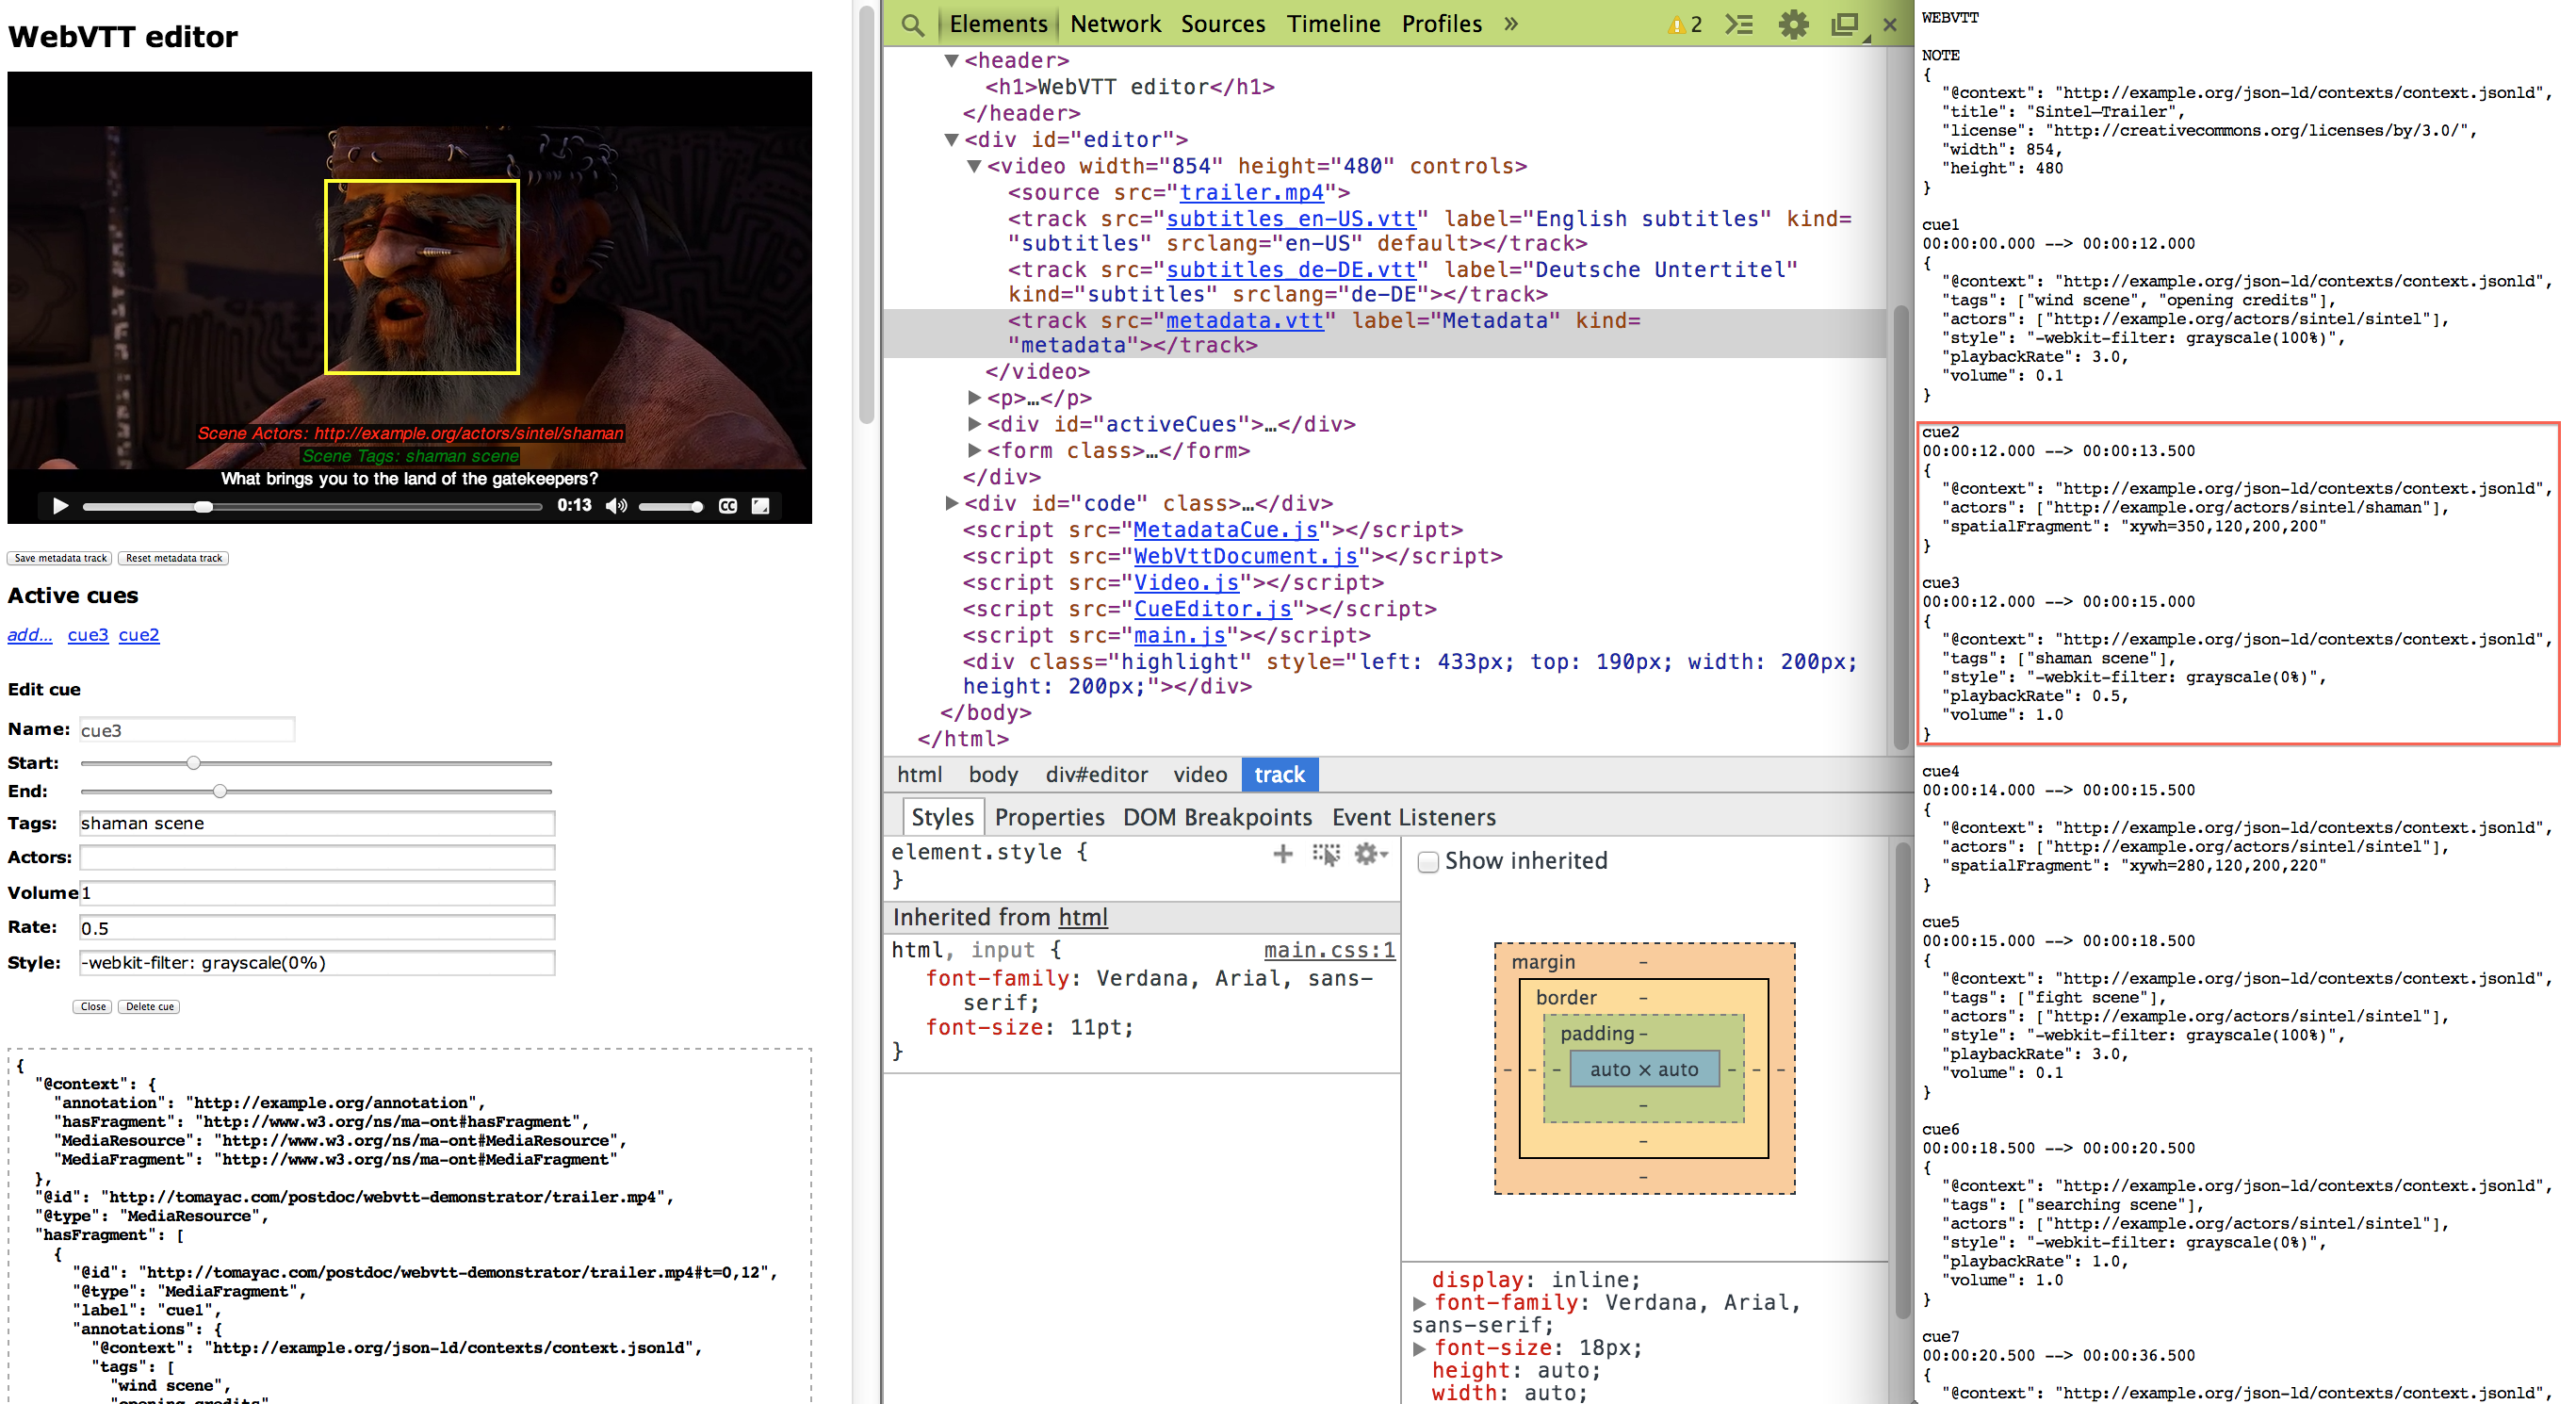
\includegraphics[width=\linewidth]{weaving-the-web(vtt)-of-data}}
  \caption{WebVTT editor interpreting the~spatiotemporal annotation ``cue2''
    that identifies the highlighted spatial fragment as \texttt{ex:actors/sintel/shaman};
    while in parallel modifying ``cue3'' with tag, volume, playback rate,
    and style (\ding{172} left: Graphical User Interface with \JSONLD\ debug view,
  \ding{173} center: Chrome Developer Tools with highlighted
  \texttt{<track src="metadata.vtt" kind="metadata">} tag,
  \ding{174} right: raw WebVTT file \texttt{metadata.vtt} with highlighted ``cue2'' and ``cue3'')}
  \label{fig:webvtt-editor}
\end{figure*}

\section{Conclusions and Future Work}

\section*{Acknowledgments}
\footnotesize
The research presented in this paper was partially supported
by the French National Agency for Research  project
\emph{Spectacle En Ligne(s)}, project reference
\mbox{ANR-12-CORP-0015}.

\normalsize
\bibliographystyle{abbrv}
\bibliography{references}

\end{document}
